\documentclass{article}
\usepackage[a4paper,margin=1in]{geometry}
\usepackage{amsmath, amssymb, amsthm}
\usepackage{xspace}
\usepackage{needspace, etoolbox}
\usepackage{url}

\usepackage{mdframed}
\usepackage{hyperref}
\usepackage{cleveref}
\usepackage{thm-restate}

\usepackage{tikz}
\usepackage{tikz-cd}
\usetikzlibrary{fit, backgrounds, calc}


% Define a new theorem style with extra space
\newtheoremstyle{spaced}
  {0pt}   % Space above (adjust to increase/decrease)
  {0pt}   % Space below (adjust to increase/decrease)
  {} % Body font (keep as default or change)
  {}        % Indent amount
  {\bfseries} % Theorem head font
  {}       % Punctuation after theorem head
  {1em}     % Space after theorem head
  {}        % Theorem head spec

\theoremstyle{spaced}

\mdfdefinestyle{myenvs}{%
  hidealllines=false,%
  nobreak=true, % comment this to allow breaking
}

\newmdtheoremenv[style=myenvs]{theorem}{Theorem}[section] % Main counter
\newmdtheoremenv[style=myenvs]{definition}[theorem]{Definition}
\newmdtheoremenv[style=myenvs]{lemma}[theorem]{Lemma}
\newmdtheoremenv[style=myenvs]{examples}[theorem]{Examples}
\newmdtheoremenv[style=myenvs]{proposition}[theorem]{Proposition}
\newmdtheoremenv[style=myenvs]{corollary}[theorem]{Corollary}


\newenvironment{reusable}[2]{%
        \restatable{#1}{#2}
        \label{#2}}
    {\endrestatable}

\title{Finitely Descriptible Properties}
\author{
Clément Michaud \\
Independent Researcher\\
\texttt{clement.michaud34@gmail.com}
}
\date{March 2025}

\begin{document}

\maketitle

\begin{center}
\begin{minipage}{0.9\textwidth}
\small
\textbf{Abstract.} In mathematics, objects are often exhibited with special properties that can be characterized by universal properties in the language of category theory. This paper analyzes the finitary nature of the transformations between such objects and proposes a framework for encoding mathematics purely through graphs, maintaining their categorical structure and universal properties.
\end{minipage}
\end{center}

\vspace{10pt}


\section{Introduction}

Mathematical objects typically arise as particular instances of universal constructions, where transformations between them preserve structure in a finitary manner. In this paper, we study how these transformations, being finitely describable, can be represented within a purely graphical framework, enabling formal reasoning in computational settings.

\section{Preliminaries}
\subsection{Categories and Universal Properties}

Category theory provides a general framework to study mathematical structures and the relationships between them. At its core lies the notion of a category, which abstracts the idea of objects and the arrows that connect them.


\begin{definition}[Category]
A \emph{category} is a collection of \emph{objects} linked by \emph{arrows} (also called \emph{morphisms}). A category has two basic properties:
\begin{itemize}
    \item The ability to compose arrows associatively.
    \item The existence of an identity arrow for each object.
\end{itemize}
We denote the set of objects of a category $\mathcal{C}$ by $\operatorname{Ob}(\mathcal{C})$ and the set of morphisms by $\operatorname{Mor}(\mathcal{C})$.
\end{definition}

Beyond merely listing objects and morphisms, categories allow us to isolate particular objects through the notion of \emph{universal properties}. Universal properties are not incidental: they are fundamental to the way mathematics is developed. Every mathematical concept that we exhibit — from basic structures like groups or sets to more complex constructions — is characterized by a universal property that selects it uniquely, up to isomorphism, among all objects sharing a given structure.

For instance, when we speak of the group of integers $(\mathbb{Z}, +)$, we are selecting, among all groups, the free group generated by a single element, characterized by its universal mapping property. Similarly, when we refer to the natural numbers, we mean the unique (up to isomorphism) initial object in the category of inductive sets: a set equipped with a distinguished element (zero) and a successor function satisfying Peano's axioms. In each case, variable declarations and structural constraints are used to exhibit an object with the desired universal property, ensuring that our mathematical constructions are canonical and unambiguous.

\begin{definition}
A \emph{universal property} characterizes an object (up to unique isomorphism) by the existence and uniqueness of morphisms satisfying certain conditions relative to other objects.
\end{definition}

In a more formal categorical setting (see, for instance, \cite{MacLane}, or the exposition in \href{https://en.wikipedia.org/wiki/Universal_property}{Wikipedia}), universal properties are often expressed via diagrams and functors:

\begin{definition}[Universal Property --- Formal]
Let \(\mathcal{C}\) be a category, and let \(F \colon \mathcal{J} \to \mathcal{C}\) be a functor from a small category \(\mathcal{J}\) into \(\mathcal{C}\). An object \(U\) in \(\mathcal{C}\) equipped with a natural transformation 
\[
\alpha \colon \Delta_U \Longrightarrow F
\]
(where \(\Delta_U\) is the functor that sends every object of \(\mathcal{J}\) to \(U\) and every morphism to the identity on \(U\)) is said to satisfy a \emph{universal property} if, for every object \(X\) in \(\mathcal{C}\) with a natural transformation \(\beta \colon \Delta_X \Longrightarrow F\), there exists a unique morphism \(\phi \colon X \to U\) in \(\mathcal{C}\) such that \(\beta\) factors through \(\alpha\) via \(\phi\). Symbolically, we require that
\[
\beta = \alpha \circ (\Delta_{\phi}),
\]
and that \(\phi\) is unique with this property.

Intuitively, \(U\) is universal if any other \(\mathcal{C}\)-object \(X\) that tries to ``map into'' the diagram \(F\) must do so by factoring uniquely through \(U\).
\end{definition}

Universal properties in this sense encapsulate constructions ranging from products and coproducts (binary or otherwise) to free objects, limits, adjoints, and more. They ensure that once such an object \((U, \alpha)\) exists, it is determined up to isomorphism. By working with universal properties, we thus obtain concise, canonical descriptions of fundamental mathematical structures.

\newpage

\section{Ideas}

\subsection{The Essence of Abstract Categories}

An \emph{abstract category} is a purely formal structure: it consists of objects and morphisms, but neither the objects nor the morphisms are assigned any intrinsic meaning. The role of an abstract category is to capture the relations between these entities without specifying the nature of the entities themselves or how the relations are realized. In contrast, an \emph{implementation} of an abstract category involves giving concrete meaning to the objects and morphisms, typically by interpreting them within a specific mathematical or applied setting. For example, familiar categories such as $\mathbf{Set}$, $\mathbf{Grp}$, or $\mathbf{Cat}$ are all implementations of abstract categories, where objects and morphisms are interpreted: in $\mathbf{Set}$, objects are sets and morphisms are functions; in $\mathbf{Grp}$, objects are groups and morphisms are group homomorphisms. Importantly, the abstract category itself serves as the most faithful and universal expression of the idea it embodies. In this sense, an abstract category satisfies a kind of \emph{universal property}: it represents the pure essence of the structure without the bias of interpretation or implementation.

\subsection{Concrete Realizations of Abstract Categories}

While an abstract category captures the pure structural essence of a mathematical idea, concrete categories provide realizations of this abstract structure by giving explicit meaning to objects and morphisms. For instance, the concept of a cyclic group can be realized concretely through the rotations of a geometric figure by $90^\circ$ increments, where the abstract elements and operations of the group are instantiated by physical rotations and compositions. These concrete categories are special in that they maintain a strong relationship to their abstract counterparts: often, there exists an \emph{isomorphic functor} between the abstract category and the concrete realization, establishing a correspondence between the two structures in both directions. However, despite this close relationship, a concrete category is not the purest expression of the idea—it carries an interpretation that the abstract category deliberately avoids. Thus, concrete categories serve as bridges between pure abstract structure and the interpreted mathematical or physical world, preserving the structural essence while embedding it within a meaningful context.

\subsection{Instances as Detailed Categories and Forgetful Functors}

At the level of concrete categories, objects acquire meaning through their interpretation. However, it is important to distinguish between an \emph{object of a given type} and an \emph{implementation} of that type. A type abstracts away all implementation details, specifying only the essential structure and properties that instances must satisfy. In contrast, an implementation is a complete object: it realizes the type, ensuring that all properties encoded by functors related to the type category are satisfied, but it also embodies additional structure arising from its concrete representation. For example, an instance of a \texttt{Shape} type might be implemented using a \texttt{Vec} or a \texttt{HashMap}, each of which carries its own internal properties and behaviors beyond those required by the abstract notion of a shape.

Formally, an implementation can be represented as a more detailed category, which connects to the type category through a \emph{forgetful functor}. This functor maps the richer structure of the implementation to the minimal structure of the type, preserving the essential properties while discarding additional details. Thus, the relationship is inherently directional: from the implementation to the type, reflecting the abstraction process. Instances not only fulfill their type’s specification but also enrich it with new properties that remain invisible at the abstract level.

\[
\begin{tikzcd}[column sep=huge]
\mathcal{C}_{\text{Abstract}} \arrow[r, leftrightarrow, "\text{isomorphic}"'] & \mathcal{C}_{\text{Type}}  \arrow[r, leftarrow, "\text{forgetful}"'] & \mathcal{C}_{\text{Instance}}
\end{tikzcd}
\]

\subsection{Outliers Relative to a Theory}

A full and faithful functor \( F: \mathcal{C} \to \mathcal{D} \) can be interpreted as a formal representation of a theory. The source category \( \mathcal{C} \) encodes the essential structure of the theory, while the codomain \( \mathcal{D} \) provides a larger context in which the theory is interpreted. In this setting, the \emph{image} of \( F \) consists of all objects and morphisms of \( \mathcal{D} \) that are captured by the theory.

Objects of \( \mathcal{D} \) that lie outside the image of \( F \) have no preimage in \( \mathcal{C} \) and thus no corresponding meaning within the theory. These objects can be regarded as \emph{outliers}: they exist within the semantic context but fall outside the syntactic reach of the theory. Outliers highlight the boundary between what is explained by the theory and what remains beyond its scope.

This phenomenon can be illustrated with a simple example. Consider a category \( \mathcal{C} \) with two objects \( A \) and \( B \), and a category \( \mathcal{D} \) with three objects \( A', B', X \). The functor \( F \) maps \( A \mapsto A' \) and \( B \mapsto B' \), preserving morphisms fully and faithfully. However, \( X \) remains untouched, serving as an outlier relative to the theory expressed by \( F \).


\begin{center}
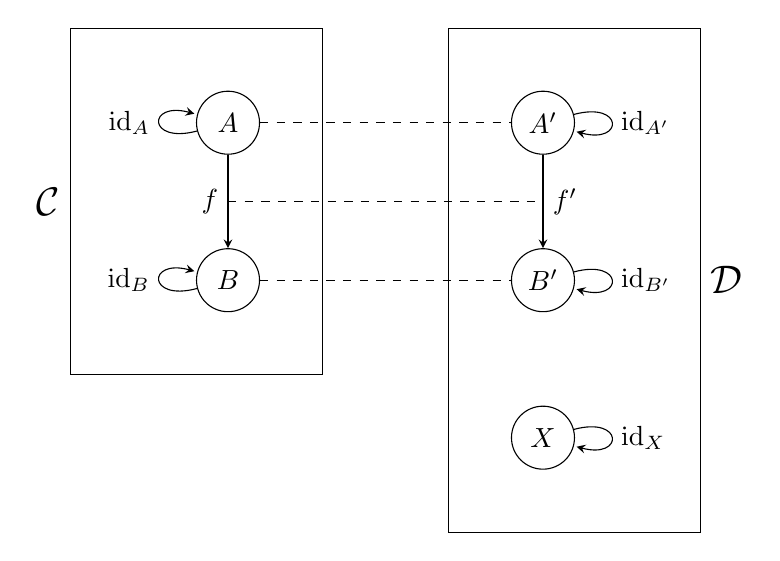
\begin{tikzpicture}[>=stealth, node distance=2cm, 
  object/.style={draw, circle, minimum size=8mm}, 
  arrow/.style={->}
]

  % Nodes for Category C
  \node[object] (A) at (0,2) {$A$};
  \node[object] (B) at (0,0) {$B$};

  % Nodes for Category D
  \node[object] (A') at (4,2) {$A'$};
  \node[object] (B') at (4,0) {$B'$};
  \node[object] (X) at (4,-2) {$X$};

  % Category C arrows
  \draw[arrow] (A) edge[loop left] node[left] {$\mathrm{id}_A$} (A);
  \draw[arrow] (B) edge[loop left] node[left] {$\mathrm{id}_B$} (B);
  \draw[arrow] (A) -- node[left] (f) {$f$} (B); % Name the midpoint of f

  % Functor F mapping objects
  \draw[dashed] (A) -- (A');
  \draw[dashed] (B) -- (B');

  % Category D arrows
  \draw[arrow] (A') edge[loop right] node[right] {$\mathrm{id}_{A'}$} (A');
  \draw[arrow] (B') edge[loop right] node[right] {$\mathrm{id}_{B'}$} (B');
  \draw[arrow] (X) edge[loop right] node[right] {$\mathrm{id}_X$} (X);
  \draw[arrow] (A') -- node[right] (f') {$f'$} (B'); % Name the midpoint of f'

  % Invisible helper coordinates to enlarge the rectangles
  \coordinate (Ctop) at ($(A) + (0,0)$);
  \coordinate (Cbottom) at ($(B) + (-0.8,0)$);
  \coordinate (Dtop) at ($(A') + (0,0)$);
  \coordinate (Dbottom) at ($(X) + (0.8,0)$);

  % Rectangle around Category C
  \node[draw, rectangle, fit=(Ctop) (Cbottom), inner sep=1.2cm, label=left:{\Large$\mathcal{C}$}] (Cbox) {};

  % Rectangle around Category D
  \node[draw, rectangle, fit=(Dtop) (Dbottom), inner sep=1.2cm, label=right:{\Large$\mathcal{D}$}] (Dbox) {};

  % Arrow from f to f'
  \draw[dashed] (f) -- node[above] {} (f');

\end{tikzpicture}
\end{center}


\subsection{Abstraction and the Loss of Internal Structure}

The concrete implementation of a type object is often far richer than the type itself. An instance may contain numerous internal properties and structures that go far beyond what is captured by the type's formal definition. As a result, the \emph{category of the implementation}—that is, the category representing all of an instance's properties and relations—is typically far too large and detailed to work with directly.

To reason effectively about such objects, it becomes necessary to \emph{abstract} away most of the implementation details, preserving only the aspects essential to the intended type. However, abstraction is a delicate process: abstracting too much leads to a collapse of structure, leaving only the bare functional relationships between types. In the extreme case, all that remains is the \emph{function signature}, representing a transformation from one type to another without any reference to internal structure.

This process mirrors the fundamental methodology of mathematics. In mathematics, we introduce variables equipped only with certain properties—such as "let \( x \) be a real number"—and intentionally disregard the internal construction or representation of these objects. By abstracting away all implementation details, mathematics achieves the remarkable ability to reason about infinite or highly complex structures using only finite expressions and finite reasoning. Abstraction is thus not only a practical necessity but also a source of mathematical power, enabling finite minds to manipulate infinite concepts.

\[
\begin{tikzcd}[column sep=huge]
\text{Rich} \arrow[r, "\text{abstraction}"] & \text{Essential} \arrow[r, "\text{abstraction}"] & \text{Minimal}
\end{tikzcd}
\]

\end{document}
